\documentclass[11pt, oneside]{article}   	% use "amsart" instead of "article" for AMSLaTeX format
\usepackage{geometry}                		% See geometry.pdf to learn the layout options. There are lots.
\geometry{letterpaper}                   		% ... or a4paper or a5paper or ... 
%\geometry{landscape}                		% Activate for for rotated page geometry
%\usepackage[parfill]{parskip}    		% Activate to begin paragraphs with an empty line rather than an indent
\usepackage{graphicx}				% Use pdf, png, jpg, or eps� with pdflatex; use eps in DVI mode
								% TeX will automatically convert eps --> pdf in pdflatex		
\usepackage{amssymb}
\usepackage{amsmath}
\usepackage{color}
\usepackage[english]{babel}

\title{Newton's Apple}
%\author{The Author}
\date{}							% Activate to display a given date or no date

\graphicspath{{/Users/telliott_admin/Dropbox/Tex/png/}}
\begin{document}

\maketitle
%\section{}
% \subsection*{R code}
% \begin{lstlisting}  \end{lstlisting}
% \begin{center} 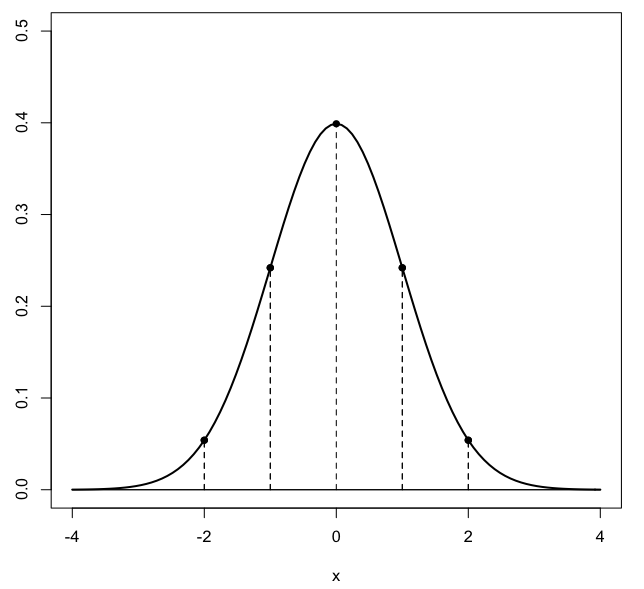
\includegraphics [scale=0.4] {gauss3.png} \end{center}
% \begin{bmatrix} a  &  b \\ c  &  d \end{bmatrix}
% \bigg |_

% this one has a wrong figure!!!

\Large
\noindent I have a short write-up about Newton's brilliant insight that gravity as observed on earth could be extended to the moon. You can read about this lots of places, I like James Gleick's \emph{Isaac Newton} (p. 55).

\begin{quote}Many years later Newton told at least four people that he had been inspired by an apple in his Woolsthorpe garden--perhaps an apple actually falling from a tree, perhaps not. He never wrote of an apple. He recalled only:

\begin{quote}\textcolor{blue}{I began to think of gravity extending to the orb of the Moon . . .}\end{quote}

---gravity as a force, then, with an extended field of influence; no cutoff or boundary---

\begin{quote}\textcolor{blue}{\& computed the force requisite to keep the Moon in her Orb with the force of gravity at the surface of the earth . . . \& found them answer pretty nearly. All this was in the two plague years of 1665-1666. For in those days I was in the prime of my age for invention \& minded mathematicks and Philosophy more than at any time since.}
\end{quote}

The apple was nothing in itself. It was half of a couple---the moon's impish twin. As an apple falls toward the earth, so does the moon; falling away from a straight line, falling around the earth.
\end{quote}

The force acting on the moon or the apple is proportional to the mass for each, but the acceleration imparted is in turn that force divided by the mass, which cancels the mass term (for apple and moon).

This leaves an equation relating the acceleration to a constant ($G$) times the mass of the earth ($M$) divided by the square of the distance to earth. 
\[ a = GM/r^2 \]
Thus, we expect that the acceleration (and the distance moved) for the moon and the apple to be in the inverse ratio as the square of their distance from the earth.

The key relationship is shown in the diagram.

\begin{center} 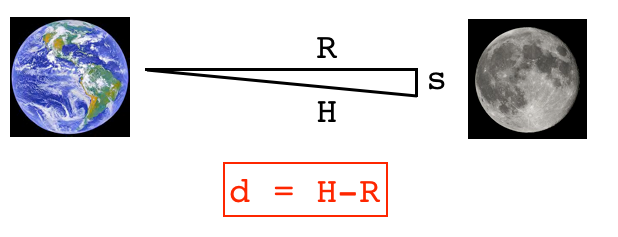
\includegraphics [scale=0.4] {newton0.png} \end{center}

We draw the tangent to the orbital circle at time-zero at a right angle with the radius. Then the distance $s$ moved in a short time, one second, is the velocity times the time. The hypotenuse, $H$, is calculated from $R$ and $s$ by the Pythoagorean Theorem. The distance "fallen" in the direction of the earth is the difference between $H$ and the radius, $R$.

So, $R = EM$ distance and $s = v_r \times 1 sec$.  Then

\[ H = \sqrt{R^2 + s^2} \]
\[ d = H - R \]

$d$ is small compared to $R$ and $H$, but it works. Using modern values for the distances:
\vspace{5 mm}

\begin{center}
  \begin{tabular}{ | l | l | } \hline
   R = EM distance (km) & $3.84$ x $10^5$ (range $3.63-4.06$) \\ \hline
   mean radius of E (km)     & $6.37$x$10^3$ (range $6.36-6.38$) \\ \hline
   ratio squared (EM dist/E radius)$^2$  & $(384/6.37)^2 = 3834$ \\ \hline
     &  \\ \hline
   T = period of orbit of M  & $27.32$ days $\times \ 86400$ sec/day$ = 2.36 \times 10^6$ sec \\  \hline
   Circumference of M orbit  & $2\pi$ x $3.84$ x $10^5$ km \\ \hline
   radial velocity of M = C/T & $1.022$ km/sec \\ \hline
   H $= \sqrt{R^2 + s^2}$ & $\sqrt{3.84 \times 10^5)^2 + (1.022)^2}=384000.00000136$ \\ \hline
   M falls in 1 sec = $H-R$         & $1.36$ mm \\ \hline
     &  \\ \hline
   earth surface gravity     & $9.8 m/s^2$ \\ \hline
   apple falls in 1 sec         & $(1/2) g t^2 = 4.9 \ m$ \\ \hline
   ratio                    & $4900 / 1.36 = 3603$  \\ \hline
   \end{tabular}
\end{center}

In the first section of the table we calculate the ratio between the moon's distance from the center of the earth and the earth's own radius.  We (and Newton) predict that the difference in force will be proportional to the square of this (3834).

From the orbital velocity of the moon and the distance to the moon we calculate that the moon travels 1 kilometer in one second and "falls" about 1.36 mm.  We compute the ratio of the distance an apple falls in one second on earth to the distance that the moon falls, and we find the ratio is about 3600.  That compares favorably with the other value.

I read somewhere that Newton first did this calculation with a value for the moon's orbital radius that was sufficiently off for him to think his result did not agree with it. Later he repeated his calculation with a more accurate value. But I can't find it now.

\end{document}  